\chapter{Training Dynamics and Optimization}

\section*{Why This Matters}

Training represents the most resource-intensive phase of model development, typically consuming 80-90\% of total project costs. Understanding training dynamics—how models converge, what drives training time, and where memory bottlenecks occur—is essential for accurate project planning, infrastructure sizing, and vendor evaluation.

The training process involves iterative parameter adjustment across millions or billions of values. Efficiency depends on algorithmic choices (optimization methods, learning rate schedules), architectural decisions (batch size, precision), and infrastructure configuration (GPU selection, distributed training strategies). Each choice presents specific trade-offs between convergence speed, resource utilization, and final model quality.

This chapter examines the technical and economic factors governing training efficiency, providing a framework for evaluating training proposals and identifying optimization opportunities.

\section*{Key Questions This Chapter Answers}

By the end of this chapter, you'll be able to answer:

\begin{itemize}
    \item Why does Adam optimizer cost 2× memory but finish training 3× faster—and when is that trade-off worth it?
    \item When does batch size become a false economy?
    \item How do you estimate training time from GPU specs and model size?
    \item What's a realistic training budget including failed experiments?
    \item How do you recognize when training dynamics indicate project failure?
\end{itemize}

\section{Mathematical Foundations: What Optimization Actually Is}

Before examining training costs and resource requirements, it's essential to understand what happens mathematically during training and why certain algorithmic choices matter.

\subsection{The Optimization Problem}

Training a neural network means finding the best values for millions or billions of parameters. "Best" means minimizing a loss function—a mathematical measure of how wrong the model's predictions are.

\textbf{Concrete Example:}

Suppose we're training a simple model with just two parameters, $w_1$ and $w_2$, to predict house prices. The loss function might be:

\begin{equation}
\text{Loss}(w_1, w_2) = \frac{1}{N} \sum_{i=1}^{N} (\text{predicted price}_i - \text{actual price}_i)^2
\end{equation}

This creates a "loss landscape"—imagine a hilly terrain where height represents prediction error. Training means finding the lowest point in this landscape.

\textbf{The Challenge:} For BERT-base with 110 million parameters, this landscape exists in 110-million-dimensional space. We can't visualize it or exhaustively search it. We need an efficient algorithm.

\subsection{Gradients: The Direction of Steepest Descent}

The \textbf{gradient} is a vector that points in the direction where the loss increases most rapidly. It tells us which direction to adjust parameters to reduce error.

\textbf{Intuitive Analogy:} Imagine you're hiking in fog and want to descend a mountain. You can't see the valley, but you can feel which direction slopes downward most steeply. The gradient is like that local slope information—it tells you which way to step.

\textbf{Mathematical Definition:} For a loss function $L(w_1, w_2, \ldots, w_n)$, the gradient is:

\begin{equation}
\nabla L = \left[\frac{\partial L}{\partial w_1}, \frac{\partial L}{\partial w_2}, \ldots, \frac{\partial L}{\partial w_n}\right]
\end{equation}

Each component tells us how much the loss changes when we adjust that specific parameter.

\textbf{Concrete Example:}

For our house price model with current parameters $w_1 = 2.0$, $w_2 = 1.5$:
\begin{itemize}
    \item Gradient component for $w_1$: -4.0 (loss decreases if we increase $w_1$)
    \item Gradient component for $w_2$: +2.0 (loss decreases if we decrease $w_2$)
\end{itemize}

To reduce loss, we adjust: $w_1 \leftarrow 2.0 + 0.1 \times 4.0 = 2.4$ and $w_2 \leftarrow 1.5 - 0.1 \times 2.0 = 1.3$

The factor 0.1 is the \textbf{learning rate}—how big a step we take.

\subsection{Backpropagation: Efficient Gradient Computation}

Computing gradients naively would require evaluating the loss function once for each parameter (110 million times for BERT-base). Backpropagation is an algorithm that computes all gradients in essentially the same time as one forward pass through the network.

\textbf{The Key Insight:} Neural networks are composed of layers, and the chain rule from calculus lets us reuse computations. If we know how the loss changes with respect to layer 12's output, we can efficiently compute how it changes with respect to layer 11's output, then layer 10, and so on.

\textbf{Why This Matters:} Backpropagation's efficiency (linear time, not exponential) is what makes training deep networks feasible. Without it, training BERT would take millions of years instead of days.

\textbf{Computational Cost:} Computing gradients via backpropagation requires approximately 2× the computation of a forward pass:
\begin{itemize}
    \item 1× for the forward pass (make predictions)
    \item 1× for the backward pass (compute gradients)
\end{itemize}

For BERT-base processing a batch, if the forward pass takes 0.1 seconds, the full training iteration (forward + backward + update) takes approximately 0.3 seconds.

\subsection{Gradient Descent: The Basic Algorithm}

The simplest optimization algorithm repeatedly:
\begin{enumerate}
    \item Compute the gradient (which direction reduces loss)
    \item Take a small step in the opposite direction (negative gradient)
    \item Repeat until loss stops decreasing
\end{enumerate}

\textbf{Pseudocode:}
\begin{verbatim}
for iteration in 1 to 1,000,000:
    gradient = compute_gradient(current_parameters)
    current_parameters = current_parameters - learning_rate * gradient
\end{verbatim}

\textbf{The Learning Rate Problem:} Too large, and you overshoot the minimum (imagine taking giant steps while descending a mountain—you might jump over the valley). Too small, and training takes forever (tiny steps mean slow progress).

\textbf{Concrete Example:}

Minimizing $f(w) = w^2$ starting from $w = 3.0$ with learning rate 0.1:
\begin{itemize}
    \item Iteration 1: gradient = 6.0, new $w$ = 3.0 - 0.1×6.0 = 2.4
    \item Iteration 2: gradient = 4.8, new $w$ = 2.4 - 0.1×4.8 = 1.92
    \item Iteration 3: gradient = 3.84, new $w$ = 1.92 - 0.1×3.84 = 1.536
    \item ... converges to $w = 0$ (the minimum)
\end{itemize}

With learning rate 0.5 (too large): $w$ oscillates wildly and never converges.
With learning rate 0.001 (too small): takes 10,000 iterations instead of 100.

\subsection{Why Adam Optimizer Matters}

Standard gradient descent uses the same learning rate for all parameters. Adam (Adaptive Moment Estimation) adapts the learning rate for each parameter individually based on gradient history.

\textbf{The Intuition:} Some parameters need large updates (they're far from optimal), while others need small updates (they're close to optimal). Adam automatically figures this out by tracking:
\begin{itemize}
    \item \textbf{First moment}: Average gradient direction (like momentum—builds up speed in consistent directions)
    \item \textbf{Second moment}: Gradient variance (parameters with noisy gradients get smaller learning rates)
\end{itemize}

\textbf{Why This Costs 2× Memory:} Adam stores two numbers per parameter (first and second moments), doubling optimizer memory from 1× parameters (standard gradient descent) to 2× parameters.

\textbf{Why It's Worth It:} Adam typically converges 2-5× faster than standard gradient descent. For a \$10,000 training run, spending \$20,000 on memory to finish in 3 days instead of 10 days is usually worthwhile—especially when iterating on experiments.

\textbf{Concrete Example:}

Training BERT-base with standard gradient descent: 25 GPU-days, \$1,500
Training BERT-base with Adam: 10 GPU-days, \$600 (despite 2× memory overhead)

The faster convergence more than compensates for the memory cost.

\section{Optimization Fundamentals}

\subsection{Gradient-Based Parameter Adjustment}

With the mathematical foundation established, we can now examine how optimization translates to training costs and resource requirements. Training optimizes model parameters through iterative gradient-based updates. The algorithm computes the direction and magnitude of parameter adjustments that reduce prediction error, then applies these adjustments across all parameters simultaneously. This process repeats thousands or millions of times until the model converges to acceptable performance.

The efficiency of this optimization depends critically on the learning rate—the scaling factor applied to computed adjustments. An appropriately calibrated learning rate enables rapid convergence. Excessive learning rates cause instability and divergence. Insufficient learning rates waste computational resources through unnecessarily slow convergence.

For transformer models, learning rates typically range from 1e-5 to 1e-3, with 1e-4 representing a common baseline. The optimal value depends on model architecture, batch size, and dataset characteristics. Empirical validation through systematic experimentation is standard practice.

\subsection{Learning Rate Impact on Training Efficiency}

Learning rate selection significantly impacts training economics. Consider three scenarios for BERT-base training:

\textbf{Learning Rate 1e-5} (suboptimal): Convergence requires approximately 50 GPU-days versus the typical 10 GPU-days. At \$2.50/GPU-hour (A100 spot pricing, 2024-2025 rates), this represents \$3,000 versus \$600—a 5× cost increase due to inefficient learning rate selection.

\textbf{Note (2026):} A100 spot pricing has decreased to approximately \$1.80-2.20/GPU-hour by 2026, with H100 spot pricing at \$3.50-4.50/GPU-hour. The cost ratios remain similar even as absolute prices decline.

\textbf{Learning Rate 1e-4} (appropriate): Standard convergence timeline of 10 GPU-days, representing baseline efficiency.

\textbf{Learning Rate 1e-3} (excessive): Training exhibits instability, potentially failing to converge. This represents complete resource waste, as unstable training produces unusable models.

\begin{figure}[htbp]
\centering
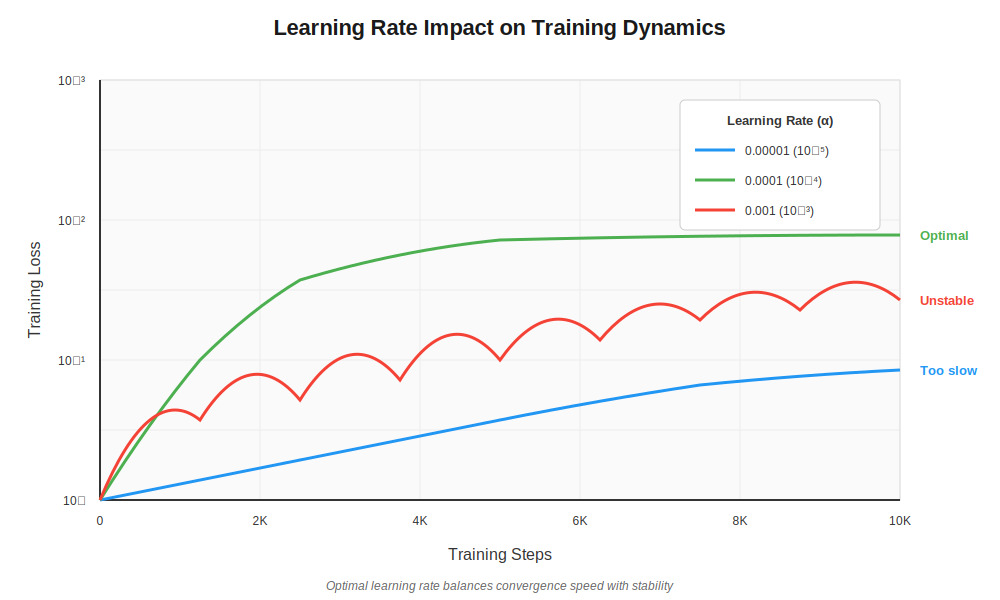
\includegraphics[width=0.9\textwidth]{chapters/diagrams/chapter02_learning_rate_curves_e5f6g7h8.pdf}
\caption{Learning rate impact on training convergence. Optimal learning rate (green) achieves efficient convergence. Suboptimal rates waste resources through slow convergence (blue) or instability (red).}
\label{fig:learning_rate}
\end{figure}

\subsection{Training Time Scaling}

Training time scales linearly with both model size and dataset size. For a model with P parameters trained on D data points:

\begin{center}
\fbox{\parbox{0.75\textwidth}{
\centering
Training Time $\propto$ P × D
}}
\end{center}

This linear relationship enables straightforward cost projection. Doubling model size doubles training time; doubling dataset size doubles training time. Doubling both quadruples training time.

For BERT-base (110M parameters, 3.3B tokens): approximately 10 GPU-days on A100 hardware. BERT-large (340M parameters, same data): approximately 40 GPU-days. GPT-2 (1.5B parameters, larger dataset): approximately 1,000 GPU-days.


\section{Training Process Architecture}

\subsection{Forward and Backward Computation}

Training consists of three phases per iteration:

\textbf{Forward Pass}: The model processes input data and generates predictions. For BERT processing a 512-token sequence, this involves converting tokens to vectors, passing through 12 transformer layers, and producing output. Computational cost is proportional to parameter count.

\textbf{Backward Pass}: The model computes parameter adjustments through backpropagation. Remarkably, this computation requires approximately the same time as the forward pass—not exponentially more, despite computing adjustments for millions of parameters. This efficiency stems from the chain rule of calculus, which enables reuse of intermediate computations.

\textbf{Parameter Update}: Computed adjustments are applied to all parameters. This is the fastest phase, involving simple arithmetic operations.

For BERT-base processing a batch of 32 sequences, one complete iteration requires approximately 0.3 seconds on A100 hardware. With 1 million iterations needed for convergence, total training time approaches 300,000 seconds (83 hours of pure compute time, approximately 10 GPU-days including overhead).

\begin{figure}[htbp]
\centering
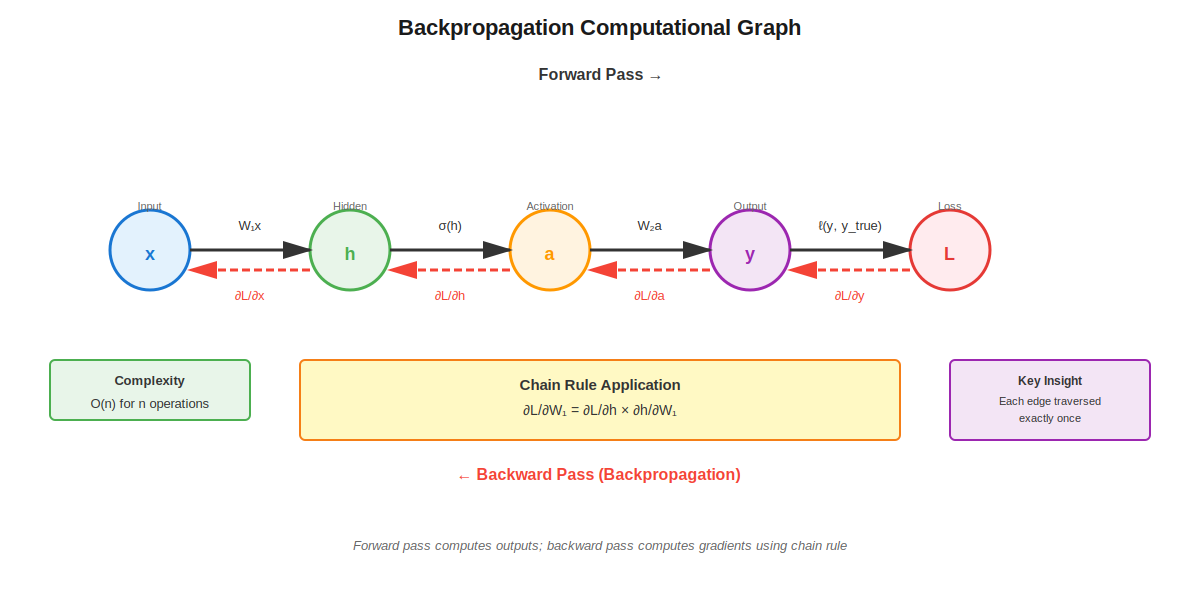
\includegraphics[width=0.95\textwidth]{chapters/diagrams/chapter02_backprop_graph_i9j0k1l2.pdf}
\caption{Training process flow showing forward pass (prediction generation) and backward pass (gradient computation). The symmetric computational cost of these phases enables linear scaling with model size.}
\label{fig:backprop_graph}
\end{figure}

\subsection{Computational Efficiency}

The linear scaling of backpropagation represents a critical efficiency property. For a model with P parameters, computing all parameter adjustments requires O(P) operations—the same order as making a prediction. This enables training of models with billions of parameters, as training time scales linearly rather than quadratically or exponentially with model size.

This efficiency has strategic implications: when evaluating proposals for larger models, training time increases proportionally to model size, not super-linearly. A 2× larger model requires approximately 2× more training time, enabling predictable cost forecasting.

\section{Memory Management}

\subsection{Training Memory Requirements}

Memory consumption during training significantly exceeds parameter storage requirements. For BERT-base (110M parameters, 440 MB storage), training requires approximately 6 GB—a 13× increase. This memory allocation includes:

\textbf{Model Parameters} (440 MB): The trained weights.

\textbf{Gradients} (440 MB): Computed parameter adjustments.

\textbf{Optimizer State} (880 MB): The Adam optimizer maintains two moving averages per parameter for adaptive learning rates, requiring 2× parameter memory.

\textbf{Activations} (3-4 GB): Intermediate layer computations stored during forward pass for use in backward pass. With batch size 32, sequence length 512, and 12 layers, activations consume approximately 60\% of total memory.

\subsection{Batch Size Trade-offs}

Batch size—the number of examples processed before parameter updates—presents a fundamental trade-off between memory consumption and computational efficiency.

\textbf{Small Batches} (8-16 sequences):
\begin{itemize}
    \item Lower memory requirements, enabling training on less expensive hardware
    \item More frequent parameter updates, potentially accelerating convergence
    \item Noisier gradient estimates, which can aid exploration but may slow convergence
    \item Poor GPU utilization, as parallel processing capabilities remain underutilized
\end{itemize}

\textbf{Large Batches} (256-512 sequences):
\begin{itemize}
    \item Higher memory requirements, necessitating expensive hardware or distributed training
    \item Fewer parameter updates per epoch, potentially slowing convergence
    \item Smoother gradient estimates, providing more stable training
    \item Efficient GPU utilization, maximizing hardware throughput
\end{itemize}

Optimal batch size for transformers typically ranges from 32-128 sequences, balancing these competing factors. The specific optimum depends on model architecture, available hardware, and convergence characteristics.

\begin{tcolorbox}[colback=green!5!white,colframe=green!75!black,title=\textbf{MENTAL MODEL: Batch Size Sweet Spot}]

\textbf{Principle:} Batch size has a U-shaped cost curve. Too small wastes GPU cycles; too large wastes memory and may slow convergence.

\textbf{The Sweet Spot (for transformers):}
\begin{itemize}
    \item Typical range: 32-128 sequences
    \item Below 32: Poor GPU utilization (less than 60\%), longer training
    \item Above 128: Diminishing returns, may require learning rate adjustment
\end{itemize}

\textbf{Decision Framework:}
\begin{enumerate}
    \item Start with batch size 32 as baseline
    \item Double batch size if GPU utilization is less than 70\%
    \item Stop when memory is 90\% full or convergence degrades
    \item If convergence degrades, increase learning rate proportionally
\end{enumerate}

\textbf{Example:} Training BERT-base on A100 (80GB). Batch size 32 uses 6GB (8\% utilization). Increase to 256 (48GB, 60\% utilization) for 3× faster training with same convergence quality.

\textbf{Red Flag:} "We use batch size 1 for stability"—this is almost never optimal. Investigate gradient accumulation or learning rate tuning instead.

\end{tcolorbox}

\subsection{Gradient Checkpointing}

Gradient checkpointing trades computation for memory by recomputing activations during backward pass rather than storing them. This technique reduces activation memory by 3-4×, enabling training of larger models or larger batches on given hardware.

The trade-off: training time increases by approximately 30-40\%. For scenarios where memory is the limiting constraint, this trade-off is favorable. For scenarios where compute is the bottleneck, gradient checkpointing is counterproductive.

Strategic application: Use gradient checkpointing when models don't fit in available memory, or when increasing batch size would improve convergence sufficiently to offset the computational overhead.

\begin{figure}[htbp]
\centering
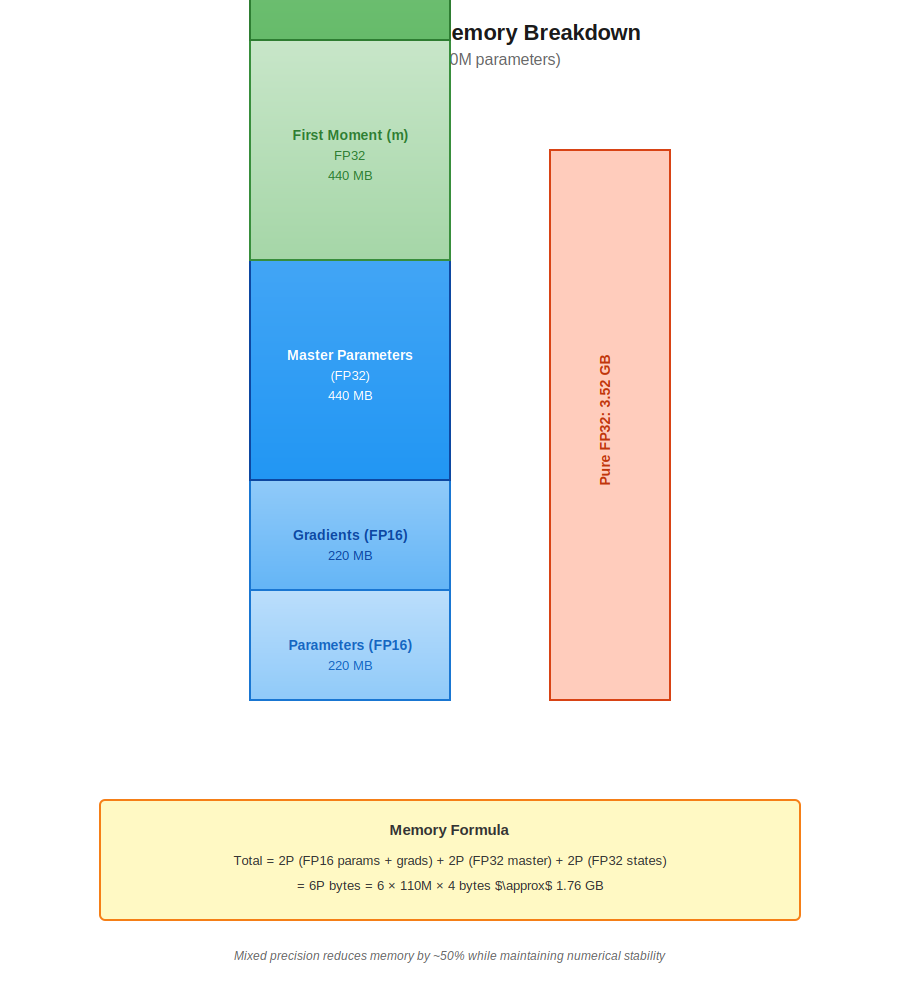
\includegraphics[width=0.9\textwidth]{chapters/diagrams/chapter02_adam_memory_m3n4o5p6.pdf}
\caption{Memory allocation during BERT-base training. Optimizer states and activations dominate memory consumption, explaining why batch size significantly impacts memory requirements.}
\label{fig:adam_memory}
\end{figure}


\section{Optimization Algorithms}

\subsection{Adam Optimizer}

The Adam (Adaptive Moment Estimation) optimizer represents the standard choice for transformer training. Adam maintains two exponential moving averages per parameter: first moment (gradient mean) and second moment (gradient variance). These statistics enable parameter-specific learning rate adaptation, accelerating convergence relative to simpler optimization methods.

The memory cost: Adam requires 2× parameter memory for these moving averages. For BERT-base, this represents an additional 880 MB. However, the convergence acceleration typically justifies this memory investment, as faster convergence reduces total training time and cost.

\textbf{Why Adaptive Learning Rates Matter: The Highway Analogy}

Standard gradient descent is like driving at a fixed speed. Steep slopes (large gradients): You want to slow down to avoid overshooting. Flat terrain (small gradients): You want to speed up to make progress.

Adam adapts the "speed" (learning rate) per parameter. Parameters with consistent gradients get confident, larger steps. Parameters with noisy gradients get cautious, smaller steps. This costs 2× memory (storing averages) but reaches good solutions 2-5× faster. For a \$10K training run, spending \$20K to finish in 3 days instead of 10 days is almost always worth it—especially when you're iterating on experiments.

\textbf{Intuition}: Adam is like cruise control that adjusts to terrain automatically, rather than you manually changing speed.

Alternative optimizers like SGD (Stochastic Gradient Descent) require less memory but converge more slowly. The trade-off analysis typically favors Adam for transformer training, as the memory cost is modest relative to activation memory, and convergence benefits are substantial.

\begin{tcolorbox}[colback=blue!5!white,colframe=blue!75!black,title=\textbf{IN PRACTICE: Choosing Between Adam and SGD}]

\textbf{Scenario}: Company training custom NLP model (BERT-scale, 110M params)

\textbf{With Adam}:
\begin{itemize}
    \item Training time: 7 days (with 8× A100s)
    \item Cost: \$5,000
    \item Convergence quality: Excellent
    \item Memory overhead: +880 MB
\end{itemize}

\textbf{With SGD} (lower memory):
\begin{itemize}
    \item Training time: 21 days (requires 3× longer to converge)
    \item Cost: \$15,000
    \item Convergence quality: Good, but requires manual tuning
    \item Memory savings: 880 MB
\end{itemize}

\textbf{Decision}: Adam is default choice. SGD memory savings ($\sim$880 MB) rarely justify 3× longer training time. Only consider SGD when memory constraints absolutely prevent Adam usage.

\end{tcolorbox}

\subsection{Mixed Precision Training}

Modern GPUs include specialized hardware for 16-bit floating-point operations, providing approximately 2× throughput relative to 32-bit operations. Mixed precision training exploits this capability by using 16-bit precision for most computations while maintaining 32-bit precision where numerical stability requires it.

Benefits:
\begin{itemize}
    \item 1.5-2× training speedup on compatible hardware (NVIDIA V100, A100, H100)
    \item 40-50\% memory reduction
    \item Minimal accuracy impact (<0.1\% typically)
\end{itemize}

\textbf{2026 Status:} Mixed precision training (FP16/BF16) is now standard practice across all major frameworks (PyTorch, TensorFlow, JAX). Most training runs use mixed precision by default. The technique is no longer considered advanced—it's baseline infrastructure.

Requirements: Modern GPU architecture with Tensor Core support. Older GPUs lack the specialized hardware necessary for mixed precision benefits.

For BERT-base, mixed precision reduces training time from 10 GPU-days to 6-7 GPU-days and memory from 6 GB to 3.5 GB. This efficiency improvement translates directly to cost reduction and faster iteration cycles.

\section{Learning Rate Schedules}

\subsection{Warmup Phase}

Transformer training employs a warmup phase: gradually increasing learning rate from near-zero to target value over initial training steps. This technique addresses optimizer initialization issues, as Adam's moving averages start at zero, making early gradient estimates unreliable.

Typical warmup duration: 10,000 steps for models trained over 1 million steps (1\% of total training). Omitting warmup frequently causes training instability or convergence to suboptimal solutions.

\subsection{Decay Schedules}

Following warmup, learning rate typically decays gradually. Cosine decay—where learning rate follows a cosine curve from peak to near-zero—represents the most common schedule. This approach enables aggressive exploration early in training and fine-tuning late in training.

\subsection{Learning Rate Schedule Impact Decomposition}

The economic impact of learning rate schedules is substantial but varies by component:

For BERT-base training (baseline = constant lr 1e-4):
\begin{itemize}
    \item Warmup (0→1e-4 over 10k steps): +5-10\% faster convergence
    \item Cosine decay (1e-4→0 over 990k steps): +15-20\% faster convergence
    \item Combined effect: +20-25\% wall-clock speedup
\end{itemize}

For larger models (GPT-2 scale):
\begin{itemize}
    \item Warmup becomes more critical: +10-15\% improvement
    \item Slower decay schedules perform better: cosine > linear > exponential
    \item Combined effect: +25-35\% wall-clock speedup
\end{itemize}

\textbf{Default recommendation for new projects}:
\begin{itemize}
    \item Linear warmup to peak\_lr over first 1\% of training
    \item Cosine decay to 10\% of peak\_lr over remaining 99\%
    \item This simple schedule achieves 95\% of benefit at minimal implementation cost
\end{itemize}

For large-scale training runs, these optimizations translate to substantial cost savings. A 25\% reduction in training time on a \$50,000 training run saves \$12,500—justifying careful schedule optimization.

\section{Cost Estimation Framework}

\subsection{Training Cost Projection}

Training costs can be estimated using:

\begin{center}
\fbox{\parbox{0.8\textwidth}{
\centering
Training Cost = (Parameters × Training Tokens) / (GPU Throughput × Efficiency) × GPU Hourly Rate
}}
\end{center}

For BERT-base:
\begin{itemize}
    \item Parameters: 110 million
    \item Training tokens: 3.3 billion
    \item GPU: A100 (312 TFLOPS)
    \item Efficiency: 40\% of peak
    \item Hourly rate: \$3
    \item Result: approximately \$720 compute cost
\end{itemize}

Including storage, networking, and overhead: approximately \$1,000 total cost for BERT-base training.

Comparative costs:
\begin{itemize}
    \item BERT-large: $\sim$\$4,000 (4× longer training)
    \item GPT-2 (1.5B parameters): $\sim$\$50,000
    \item GPT-3 (175B parameters): $\sim$\$5 million
\end{itemize}

\subsection{Efficiency Optimization}

Most training implementations can achieve 2-3× efficiency improvements through:
\begin{itemize}
    \item Mixed precision training (1.5-2× speedup on compatible hardware)
    \item Batch size optimization for available hardware
    \item Gradient accumulation to simulate larger batches without memory increase
    \item Data loading optimization to eliminate I/O bottlenecks
\end{itemize}

For large-scale training runs, these optimizations translate to substantial cost reductions. A 2× efficiency improvement on a \$50,000 training run saves \$25,000—justifying significant engineering investment in training infrastructure.

\section{Evaluation Framework}

\subsection{Training Proposal Assessment}

When evaluating training proposals, consider:

\textbf{Resource Estimates}:
\begin{itemize}
    \item What is the estimated training time in GPU-hours, and how was it calculated?
    \item Does the estimate account for warmup, learning rate schedules, and convergence criteria?
    \item What contingency is included for failed runs or hyperparameter tuning?
\end{itemize}

\textbf{Optimization Strategy}:
\begin{itemize}
    \item What learning rate and schedule are proposed? What is the empirical justification?
    \item What batch size is planned? Is it constrained by memory or convergence considerations?
    \item Is mixed precision training employed? What speedup is expected?
\end{itemize}

\textbf{Monitoring and Validation}:
\begin{itemize}
    \item What metrics will indicate successful training? What constitutes convergence?
    \item What is the checkpointing strategy? How will progress be preserved against failures?
    \item What is the plan for addressing training instability if it occurs?
\end{itemize}

\subsection{Common Assessment Pitfalls}

\textbf{Insufficient Warmup}: Omitting or inadequately sizing warmup phases frequently causes training instability. Proposals should include explicit warmup specifications.

\textbf{Inappropriate Learning Rates}: Learning rates should be justified through preliminary experiments or reference to comparable models. Arbitrary learning rate selection often leads to inefficient training or failure.

\textbf{Memory Constraint Neglect}: Proposals should explicitly address memory requirements and verify feasibility on available hardware. Out-of-memory failures waste all invested resources.

\textbf{Inadequate Checkpointing}: Hardware failures occur. Without regular checkpointing (every 2-4 hours minimum), training progress is lost. Checkpoint strategy should be explicit in proposals.

\begin{tcolorbox}[colback=red!5!white,colframe=red!75!black,title=\textbf{CAUTIONARY TALE: Training That Took 10× Longer Than Estimated}]

\textbf{What Happened:}

An e-commerce company decided to train a recommendation transformer from scratch. Initial estimate: 5 days on 8× A100 GPUs (\$10K). They calculated based on theoretical FLOPS and model size.

\textbf{Day 3:} Training loss barely decreased. GPU utilization averaged 25\%. Investigation revealed multiple issues: Batch size too small (8) for A100 memory capacity (80GB)—wasting 90\% of available memory. Learning rate not tuned—using default 1e-4 when 5e-4 would converge 3× faster. No learning rate warmup—caused initial instability requiring restart. Data pipeline bottleneck—GPUs idle 40\% of time waiting for data.

\textbf{Week 6:} After fixes, training finally converged. Total time: 42 days. Total cost: \$84K (8.4× over budget).

\textbf{Outcome:}

Project nearly cancelled. Post-mortem revealed they ignored: GPU utilization analysis (should be greater than 70\%). Learning rate validation experiments (2-3 days, \$500 investment would have saved \$70K). Data pipeline profiling (revealed bottleneck immediately). Batch size optimization (could have used batch size 128, 16× faster).

\textbf{Lesson:} Theoretical FLOPS calculations ignore real-world bottlenecks. Always profile before scaling. GPU utilization below 60\% indicates optimization opportunities. Learning rate tuning is not optional—it's the difference between 5 days and 42 days. Data pipeline speed must match GPU consumption rate.

\textbf{What They Should Have Done:}
\begin{enumerate}
    \item Run 1-day pilot with profiling (cost: \$250)
    \item Identify bottlenecks (data pipeline, batch size, learning rate)
    \item Fix issues before full training run
    \item Realistic estimate: 7 days, \$14K (still 40\% over initial estimate but 6× cheaper than actual)
\end{enumerate}

\textbf{Red Flag:} "We calculated training time from FLOPS"—this ignores memory bandwidth, data loading, optimizer overhead, and convergence dynamics. Always validate with pilot runs.

\end{tcolorbox}

\section{Where You'll See This in Practice}

Training dynamics determine whether AI projects succeed on time and on budget. Here's how Chapter 2's concepts appear in real domain applications:

\subsection{Drug Discovery (Chapter 12.5)}

Molecular property prediction models face small datasets (10K-100K molecules) requiring careful learning rate schedules (Section 2.5), long training times (weeks) where optimizer choice (Section 2.4.1) determines project feasibility, and high cost per failed experiment—warmup phase (Section 2.5.1) prevents wasted GPU-days.

\textbf{Real scenario}: Pharmaceutical company trains generative model for drug candidates. Training cost: \$50K. Without proper learning rate warmup (Section 2.5.1), training diverged after 3 days (\$15K wasted). Second attempt with warmup succeeded.

\textbf{Decision point}: Your team proposes 100 training experiments for hyperparameter search. Section 2.6's cost estimation framework reveals this would cost \$500K. Question: Can we reduce search space or use cheaper proxy tasks?

\subsection{Financial Risk Models (Chapter 14.2)}

Credit risk transformers require batch size optimization (Section 2.3.2) for class-imbalanced datasets (95\% non-default, 5\% default), memory management (Section 2.3) when training on sensitive data that can't leave secure environment, and cost justification (Section 2.6) when traditional ML (XGBoost) might suffice.

\textbf{Real scenario}: Bank proposed TabTransformer for credit scoring. Analysis using Section 2.6 frameworks: Training cost: \$20K (10 GPU-days). Expected lift: 2\% AUC improvement. Value: \$500K/year reduced defaults. ROI: 25× in year 1, approved.

\textbf{Decision point}: Vendor quotes "10 GPU-days" for training. Section 2.6.1 helps you verify: Are they counting failed experiments? Hyperparameter tuning? Batch size is appropriate for their GPU memory?

\subsection{Customer Support Bots (Chapter 10.3)}

Fine-tuning conversational models involves deciding between full fine-tuning versus LoRA (Section 2.4—memory trade-offs), estimating retraining frequency as customer questions evolve (Section 2.6 cost projection), and managing drift when training distribution differs from production (Section 2.7.1).

\textbf{Real scenario}: Support team wants to fine-tune GPT-3.5 on 50K ticket pairs. Full fine-tuning: \$5K, 8 hours. LoRA (low-rank adaptation): \$500, 2 hours, 4× less memory. Retraining quarterly: \$2K/year (LoRA) versus \$20K/year (full). Decision: Use LoRA—10× cheaper for negligible accuracy difference.

\textbf{Decision point}: Section 2.4's optimizer analysis helps you evaluate whether the memory overhead is justified by faster convergence.

\subsection{Legal Document Review (Chapter 13.1)}

Contract analysis models face limited training data (legal documents are confidential and expensive to label), overfitting risks (Section 2.7.2) with small datasets, and high accuracy requirements (99\%+) demanding careful training monitoring (Section 2.7).

\textbf{Real scenario}: Law firm trains contract clause extraction model on 5K labeled contracts. Initial attempt: Training loss decreased but validation accuracy plateaued at 85\%. Root cause (Section 2.7.1): Model memorizing training data, not generalizing. Solution: Smaller model plus aggressive regularization plus data augmentation (Chapter 8.3). Result: 92\% accuracy, still below 99\% requirement, ruled out pure ML approach.

\textbf{Decision point}: Section 2.7's evaluation framework helps you recognize when training dynamics indicate the problem isn't solvable with current data/architecture.

\subsection{Code Generation (Chapter 11)}

Training code completion models involves massive datasets (billions of tokens from GitHub) requiring distributed training (Section 2.6.2), context length trade-offs (how much code history to include?) affecting memory (Section 2.3), and continuous retraining as programming practices evolve (Section 2.6 cost projection).

\textbf{Real scenario}: Company considers training custom code model versus using Copilot API. Custom training: \$200K initial plus \$20K/quarter retraining. Copilot API: \$50K/year at current usage. Break-even: 6× usage increase or 3 years with 2× annual growth. Decision: Start with API, plan migration at 5M requests/month.

\textbf{Decision point}: Section 2.6's cost estimation framework helps you calculate TCO over 3 years, not just immediate costs.

\subsection{Key Patterns Across Domains}

\textbf{Training Cost Dominates When}: Frequent retraining required (customer support, fraud detection), hyperparameter search needed (new problem domains), or data distribution shifts rapidly (financial markets, breaking news).

\textbf{Training Cost Is One-Time When}: Stable problem domain (medical image classification), high inference volume (search engines, recommendation systems), or pre-trained models suffice with minimal fine-tuning.

Use Section 2.6's frameworks to identify which category your use case falls into—this determines whether training optimization is critical or irrelevant to your ROI.

\subsection{Decision Checklist: When Evaluating Training Proposals}

Before approving training budget, verify: Training time estimate includes failed experiments (typically 3-5× successful runs). Memory requirements account for activations plus gradients plus optimizer state (Section 2.3.1). Batch size is appropriate for available GPU memory (Section 2.3.2). Learning rate schedule includes warmup (Section 2.5.1). Validation strategy prevents overfitting (Section 2.7.1). Cost estimate spans full hyperparameter search, not single run (Section 2.6.1).

\textbf{Red flags}: "We'll know the final cost after we start" (No cost ceiling defined). Batch size exceeds GPU memory capacity (Training won't run). No validation set mentioned (Overfitting guaranteed). Linear cost scaling assumed (Ignores hyperparameter search overhead).

This checklist, grounded in Chapter 2's concepts, will save you from approving underfunded or poorly-planned training projects.

\section{Key Insights}

\textbf{Linear Scaling}: Training time scales linearly with model size and dataset size, enabling predictable cost forecasting. A 2× larger model requires approximately 2× more training time.

\textbf{Memory Dominance}: Activation memory typically consumes 60\% of training memory, with batch size as the primary control lever. Memory constraints often limit training before computational constraints.

\textbf{Learning Rate Criticality}: Appropriate learning rate selection can reduce training time by 5× or more. Systematic learning rate validation is essential for efficient training.

\textbf{Adam Justification}: Adam's 2× memory overhead is typically justified by convergence acceleration. The memory cost is modest relative to activation memory.

\textbf{Mixed Precision Benefits}: On compatible hardware, mixed precision provides 1.5-2× speedup with minimal accuracy impact. This represents a substantial efficiency gain for minimal implementation cost.

\textbf{Optimization ROI}: Training efficiency improvements of 2-3× are achievable through systematic optimization. For large-scale training, this justifies significant engineering investment.

The next chapter examines attention mechanisms—the architectural innovation enabling transformer models—and their computational characteristics.

